\section{Supplementary Experiments}
\label{app:supplementary-experiments}

In this appendix, rows labeled ``baseline UCC'' are frozen-control rows:
they denote the upstream UCC v0.4.12 pre-semantic default path defined in the
provenance map of Appendix~B, not a separate semantic method.

\subsection{Exact-Semantics Witness Data}
\label{app:witness-data}

The following tables contain the full uniform-600\,s comparison data for
the exact-semantics witnesses discussed in
\cref{cor:exact-semantics-corollary} of the main text.

\begin{table*}[htbp]
\centering
\scriptsize
\resizebox{\textwidth}{!}{%
\begin{tabular}{cccccccc}
\toprule
Requested & Actual & semantic UCC & \texttt{qiskit opt3} & PyZX \texttt{full\_reduce} & TKET PauliSimp (rebased) & staq rotation folding & TKET GuidedPauliSimp \\
\midrule
4{,}000 & 3{,}998 & 42/24/12 & 9588/5593/4788 & 107/59/31 & 52/29/19 & 9188/4996/4788 & 13574/6392/4788 \\
10{,}000 & 9{,}998 & 42/24/12 & 23988/13993/11988 & timeout & 62/36/28 & 22988/12496/11988 & 33974/15992/11988 \\
20{,}000 & 19{,}998 & 42/24/12 & 47988/27993/23988 & timeout & 59/27/20 & 45988/24996/23988 & 67974/31992/23988 \\
50{,}000 & 49{,}998 & 42/24/12 & 119988/69993/59988 & timeout & 73/44/35 & 114988/62496/59988 & 169974/79992/59988 \\
100{,}000 & 99{,}998 & 42/24/12 & 239988/139993/119988 & timeout & 66/37/28 & 229988/124996/119988 & 339974/159992/119988 \\
\bottomrule
\end{tabular}%
}
\caption{Uniform-600\,s comparison on the rational CP finite-range
witness. Completed cells report gates/depth/cx; other entries are status
outcomes and are not scored as structural wins. The family is certified
only for $R < T = 131040$, with per-transducer tail constants. No
external row is a formal theorem instance.}
\label{tab:rational-cp-600}
\end{table*}

\begin{table*}[htbp]
\centering
\scriptsize
\resizebox{\textwidth}{!}{%
\begin{tabular}{cccccccc}
\toprule
Requested & Actual & semantic UCC & \texttt{qiskit opt3} & PyZX \texttt{full\_reduce} & TKET PauliSimp (rebased) & staq rotation folding & TKET GuidedPauliSimp \\
\midrule
4{,}000 & 3{,}998 & 27/18/6 & 4799/2801/2394 & 38/19/8 & 36/14/6 & 3402/2201/2394 & 8786/4000/2394 \\
10{,}000 & 9{,}998 & 27/18/6 & 12000/7001/5994 & 48/33/12 & 35/15/8 & 8502/5501/5994 & 21986/10000/5994 \\
20{,}000 & 19{,}998 & 27/18/6 & 24000/14001/11994 & correctness failure & 38/16/8 & 17002/11001/11994 & 43986/20000/11994 \\
50{,}000 & 49{,}998 & 27/18/6 & 60000/35001/29994 & timeout & 36/15/8 & 42502/27501/29994 & 109986/50000/29994 \\
100{,}000 & 99{,}998 & 27/18/6 & 120000/70001/59994 & timeout & 37/16/8 & 85002/55001/59994 & 219986/100000/59994 \\
\bottomrule
\end{tabular}%
}
\caption{Uniform-600\,s comparison on the irrational independent-Pauli
witness. Completed cells report gates/depth/cx; other entries are status
outcomes and are not scored as structural wins. The exact rank and
irrational-angle certificate, rather than this numerical table,
instantiate \cref{cor:exact-semantics-corollary}.}
\label{tab:irrational-600}
\end{table*}

\subsection{Fourier Witness Diagnostics}

The tables in this subsection support the main-text Fourier witness without
serving as additional theorem instances. The canonical theorem-linked CP
witness is the finite-range case in \cref{tab:rational-cp-600}; the
generalized topology/angle rows are robustness diagnostics, and the external
stress rows use the budgets recorded in their frozen source files.

\begin{table*}[htbp]
\centering
\scriptsize
\begin{tabularx}{\textwidth}{@{}lccccX@{}}
\toprule
Topology & Angles & Points & \texttt{qiskit} ok/TO & Semantic completed & Semantic output signatures \\
\midrule
chain CP & 3 & 12 & 9 / 3 & all 12 & 23--27 gates, 17--18 depth, 6 \texttt{cx} \\
ring CP & 3 & 12 & 9 / 3 & all 12 & 32 gates, 23 depth, 8 \texttt{cx} \\
sparse CP $0.5$ & 3 & 12 & 6 / 6 & all 12 & 25--27 gates, 11--12 depth, 6 \texttt{cx} \\
full-pair CP & 2 & 6 & 4 / 2 & all 6 & 42 gates, 24 depth, 12 \texttt{cx} \\
\midrule
Total points & -- & 42 & 28 / 14 & all rows & repetition-independent at fixed topology/angle \\
\bottomrule
\end{tabularx}
\caption{Generalized fixed-width Fourier witness suite. Each point is a paired run of semantic UCC and \texttt{qiskit opt3} on an $H D^r H$ circuit at $n=4$, with requested sizes up to $50$k gates. The rows are filtered from the recorded 284-row generalized suite by the $n=4$ topology/angle/size slice. Recorded \texttt{qiskit opt3} timeout cells in that source use legacy 60\,s or 90\,s budgets, so the table is a robustness diagnostic rather than a uniform-600\,s comparison.}
\label{tab:generalized-fourier-witness}
\end{table*}

\begin{table}[htbp]
\centering
\scriptsize
\setlength{\tabcolsep}{2pt}
\begin{tabular}{cccccc}
\toprule
Width ($n$) & Checks & Output Gates & Depth & CX Count & Seed Variance \\
\midrule
4 & 15 / 15 & 42 & 24 & 12 & 0 \\
5 & 15 / 15 & 65 & 32 & 20 & 0 \\
6 & 15 / 15 & 93 & 40 & 30 & 0 \\
\bottomrule
\end{tabular}
\caption{Correctness and seed-robustness certificate for the full-pair Fourier witness. The correctness experiment checks $3$ widths $\times$ $3$ requested sizes $\times$ $5$ angle seeds using Qiskit \texttt{Operator.equiv}; all $45$ configurations are equivalent to the original circuit up to global phase. The seed-robustness experiment contains $90$ rows including \texttt{qiskit opt3}; semantic UCC has zero output gate-count variance across the five tested nonresonant angle seeds at each width.}
\label{tab:fourier-correctness-seed}
\end{table}

\begin{table*}[tbp]
\centering
\scriptsize
\begin{tabularx}{\textwidth}{@{}>{\raggedright\arraybackslash}Xccc
  >{\raggedright\arraybackslash}X
  >{\raggedright\arraybackslash}X@{}}
\toprule
Method & Requested & Actual & Status & Gates/depth/\texttt{cx} & Certificate \\
\midrule
semantic UCC (Fourier-layer IR enabled) & 100{,}000 & 99{,}998 & completed & 42/24/12 & \texttt{Operator.equiv=True} \\
phase-polynomial reference & 100{,}000 & 99{,}998 & completed & 42/24/12 & \texttt{Operator.equiv=True} \\
\bottomrule
\end{tabularx}
\caption{Large-instance correctness extension on the canonical $n=4$, $r=9999$ Fourier witness. The check is a finite-instance Qiskit \texttt{Operator.equiv} certificate for the two completed compressed outputs only; it does not certify the generalized topology/angle suite or prove an algebraic identity for all $r$.}
\label{tab:large-correctness-extension}
\end{table*}

\begin{table*}[t]
\centering
\scriptsize
\begin{tabular}{@{}rrrrrr@{}}
\toprule
Width & Requested & semantic UCC & \texttt{qiskit opt3} & PyZX bridge & TKET FullPeephole \\
\midrule
5 & 4{,}000 & 65 & 11{,}711 & 14{,}640 & 30{,}369 \\
5 & 10{,}000 & 65 & 29{,}315 & 36{,}640 & timeout \\
6 & 4{,}000 & 93 & 12{,}108 & 15{,}321 & 33{,}881 \\
6 & 10{,}000 & 93 & 30{,}417 & 38{,}487 & timeout \\
\bottomrule
\end{tabular}
\caption{Representative external stress tests on the width-axis full-pair Fourier witness. Entries report output gates after the configured bridge pipeline and final target-basis compilation. PyZX completes all four runs but does not recover the bounded semantic forms $65$ and $93$; TKET completes the $4$k runs with larger outputs and times out at $10$k. The recorded budget in this stress file is 300\,s.}
\label{tab:width-axis-external-stress}
\end{table*}

\begin{table*}[tbp]
\centering
\scriptsize
\begin{tabular}{@{}lrrrr@{}}
\toprule
Topology & semantic UCC & \texttt{qiskit opt3} & PyZX bridge & TKET FullPeephole \\
\midrule
chain CP & 27 & $6{,}851$ / $17{,}136$ & $10{,}838$ / $27{,}121$ & $20{,}555$ / timeout \\
ring CP & 32 & $7{,}996$ / $19{,}996$ & $11{,}984$ / $29{,}984$ & $23{,}987$ / $59{,}987$ \\
sparse CP $0.5$ & 27 & $6{,}851$ / $17{,}136$ & $10{,}838$ / $27{,}121$ & timeout / timeout \\
full-pair CP & 42 & $10{,}783$ / $26{,}983$ & $13{,}574$ / $33{,}974$ & timeout / timeout \\
\bottomrule
\end{tabular}
\caption{Topology-axis external stress test at $n=4$ with nonresonant seed $0$. Each external-baseline cell reports output gates at requested sizes $4$k / $10$k. The deterministic sparse-CP draw uses the same number of CP edges as chain CP and is graph-isomorphic to a chain at $n=4$, which explains the matching \texttt{qiskit opt3} and PyZX gate totals for those two rows. The recorded budget in this stress file is 300\,s.}
\label{tab:topology-external-stress}
\end{table*}

\begin{table*}[t]
\centering
\scriptsize
\begin{tabularx}{\textwidth}{@{}>{\raggedright\arraybackslash}p{0.18\textwidth}
                >{\raggedright\arraybackslash}p{0.19\textwidth}
                >{\raggedright\arraybackslash}X
                >{\raggedright\arraybackslash}p{0.19\textwidth}@{}}
\toprule
Pipeline & Representation tested & Observed behavior in the disclosed suites & Interpretation \\
\midrule
semantic UCC (Fourier-layer IR enabled)
& pre-basis Fourier-layer term
& completed 5/5; $42$ gates, depth $24$, $12$ \texttt{cx} at every tested scale
& semantic side \\
phase-polynomial reference
& same Qiskit input; only commuting-diagonal coefficient aggregation
& completed 5/5; $42$ gates, depth $24$, $12$ \texttt{cx} at $4$k--$100$k
& authors' protocol-specific constructive control \\
\texttt{qiskit opt3}
& preset target-basis pipeline
& completed 5/5; grows from $9{,}588$ gates at $4$k to $239{,}988$ gates at $100$k
& strong completed baseline, but not bounded \\
PyZX configured bridge
& Qiskit--QASM--PyZX basic optimization--Qiskit
& completed 4/5; grows through $169{,}974$ gates at $50$k and times out at $100$k
& configured bridge does not recover bounded form \\
PyZX \texttt{full\_reduce}
& QASM to PyZX graph; \texttt{full\_reduce}; extract and lower
& rational witness: completes only at $4$k with $107$ gates, depth $59$, $31$
\texttt{cx}; timeout at $10$k--$100$k. Irrational witness: completes and
validates at $4$k and $10$k with $38$ and $48$ gates; correctness failure at
$20$k; timeout at $50$k and $100$k
& strong small-scale simplification; correctness failure remains distinct from timeout and error \\
TKET FullPeephole
& direct Qiskit--TKET bridge to FullPeepholeOptimise
& timeout on all five canonical sizes under the 600\,s budget
& no completed bounded recovery in this protocol \\
TKET PauliSimp (unrebased configuration)
& direct Qiskit--TKET bridge to PauliSimp
& predicate error on all five sizes for both witness families
& provenance-only configuration; not a structural loss \\
TKET PauliSimp (rebased)
& generic DecomposeBoxes, AutoRebase to \{CX,Rz,Rx\}, RemoveRedundancies,
PauliSimp, RemoveRedundancies
& completes and validates at all five scales: $52$--$73$ gates on the rational
witness and $35$--$38$ on the irrational witness
& generic aggregate reconstruction crosses the formal boundary \\
staq rotation folding
& generic target-basis QASM2 through public \texttt{fold\_rotations}
& completes and validates at all five scales, but grows from $9{,}188$ to
$229{,}988$ gates on the rational witness and from $3{,}402$ to $85{,}002$ on
the irrational witness
& completed public baseline; growing output is not an impossibility result \\
TKET GuidedPauliSimp
& direct Qiskit--TKET bridge to GuidedPauliSimp
& completed 5/5 on each witness; grows from $13{,}574$ to $339{,}974$ gates on
the rational witness and from $8{,}786$ to $219{,}986$ on the irrational witness
& successful pipeline, but not bounded \\
artifact UCC (Fourier-layer IR disabled)
& same artifact with Fourier-layer semantic path disabled
& in ablation/resource runs, completes at $4$k, $10$k, and $20$k with $9{,}588$, $23{,}988$, and $47{,}988$ gates; times out at $50$k and $100$k
& semantic-path causality check; completed rows materialize large outputs \\
\bottomrule
\end{tabularx}
\caption{External-pipeline status matrix and constructive controls for the
rational CP and irrational independent-Pauli witnesses. Completed outputs and
status outcomes are separated. The rebased and unrebased PauliSimp
configurations are distinct, and no row is treated as a formal transducer
instance.}
\label{tab:external-failure-matrix}
\end{table*}

\subsection{Controlled Fixed-Basis Results}

\subsubsection{\texorpdfstring{Repeated $\mathrm{QFT}+\mathrm{QFT}^{-1}$ ($100$k gates)}{Repeated QFT+inverse-QFT (100k gates)}}

\subsubsection{\texorpdfstring{Repeated $\mathrm{QFT}+\mathrm{QFT}$ control ($100$k gates)}{Repeated QFT+QFT control (100k gates)}}

\begin{table*}[!t]
\centering
\begin{tabular}{lrr rr}
\toprule
& \multicolumn{2}{c}{$\mathrm{QFT}+\mathrm{QFT}^{-1}$}
& \multicolumn{2}{c}{$\mathrm{QFT}+\mathrm{QFT}$} \\
\cmidrule(lr){2-3}\cmidrule(lr){4-5}
Method & Output Gates & Output Depth & Output Gates & Output Depth \\
\midrule
translation only & 400{,}000 & 142{,}500 & 400{,}000 & 140{,}000 \\
baseline UCC & 968{,}784 & 276{,}266 & 1{,}207{,}504 & 317{,}501 \\
semantic UCC & 0 & 0 & 347{,}500 & 125{,}000 \\
\bottomrule
\end{tabular}
\caption{Controlled fixed-basis results for the repeated inverse and
non-inverse QFT controls at 100k input gates.}
\label{tab:qft-inverse-fixed}
\label{tab:qft-control-fixed}
\end{table*}

These finite controls show that, for this configured family and the tested
pipelines, a large structural opportunity remains after controlling for the
final target basis.  They are not a separate theorem-level witness.


\subsubsection{Systematic \texorpdfstring{$\mathrm{QFT}+\mathrm{QFT}^{-1}$}{QFT+inverse-QFT} external scaling}

The inverse-QFT scaling control is not the primary theorem witness, because
\texttt{qiskit opt3} also finds the zero-gate circuit at smaller sizes. Its role
is to test scalability when both paths return the same zero-gate output. As shown in
\cref{tab:qft-inverse-external-scaling}, the semantic artifact returns the
zero-gate circuit at all tested sizes, is faster than \texttt{qiskit opt3}
wherever \texttt{qiskit opt3} completes, and avoids the \texttt{qiskit opt3}
timeouts at $50$k and $100$k. As an additional control, it also matches
\texttt{qiskit\_commutative\_inverse} in output quality and is faster at every
tested size.

\begin{table*}[htbp]
\centering
\small
\begin{tabular}{rrrrrr}
\toprule
Input gates & \multicolumn{2}{c}{\texttt{qiskit opt3}} & \multicolumn{2}{c}{\texttt{qiskit\_commutative\_inverse}} & semantic UCC \\
\cmidrule(lr){2-3}\cmidrule(lr){4-5}
 & Gates & Runtime & Gates & Runtime & Runtime \\
\midrule
4{,}000 & 0 & 1.052 s & 0 & 0.082 s & 0.063 s \\
10{,}000 & 0 & 6.090 s & 0 & 0.182 s & 0.124 s \\
20{,}000 & 0 & 24.596 s & 0 & 0.341 s & 0.279 s \\
50{,}000 & timeout & $>90$ s & 0 & 0.979 s & 0.829 s \\
100{,}000 & timeout & $>90$ s & 0 & 2.271 s & 1.651 s \\
\bottomrule
\end{tabular}
\caption{External scaling on repeated $\mathrm{QFT}+\mathrm{QFT}^{-1}$. The semantic UCC artifact returns zero gates at all tested sizes; the table reports runtime because output quality is identical to the zero-gate reference wherever the references complete. Timeout cells in this source use the recorded 90\,s budget.}
\label{tab:qft-inverse-external-scaling}
\end{table*}


\subsection{Why Simple Pass Reordering Is Not Enough}

To test whether the observed gains are mainly explained by a missing pass or
pass-ordering issue inside \texttt{UCCDefaults}, we ran a controlled comparison
between baseline UCC, several minimal \texttt{UCCDefaults}-style alternatives,
and the semantic artifact. The minimal alternatives were
\texttt{defaults\_preinverse\_only}, \texttt{defaults\_reordered\_only}, and
\texttt{defaults\_minimal\_bundle}; the all-to-all cases were normalized to the
same final target basis $B = [\texttt{cx},\texttt{rx},\texttt{ry},\texttt{rz},\texttt{h}]$,
and the backend-aware cases used fixed transpiler seed $12345$. This is a
separate reorder-probe experiment, so its runtime numbers should be read
independently from the frozen mainline tables below.  Its hardware rows have
reader labels \texttt{RP23-qpeexact-s12345-c89463b96} and
\texttt{RP23-qaoa-s12345-c89463b96}; the canonical hardware campaign below
instead uses the \texttt{HW24-...-c0f32747f} labels.  The differing labels are
different full experiment keys, not repeated measurements of one row.

\begin{table*}[t]
\centering
\scriptsize
\begin{tabular}{llrrrr}
\toprule
Case & Method & Gates & Depth & CX count & Runtime \\
\midrule
\multirow{6}{*}{\texttt{phase\_estimation\_real}}
  & baseline UCC & 471{,}819 & 328{,}271 & 58{,}491 & 75.538 s \\
  & \texttt{defaults\_preinverse\_only} & 485{,}780 & 332{,}924 & 82{,}925 & 80.045 s \\
  & \texttt{defaults\_reordered\_only} & 485{,}780 & 332{,}924 & 82{,}925 & 80.005 s \\
  & \texttt{defaults\_minimal\_bundle} & 485{,}780 & 332{,}924 & 82{,}925 & 80.084 s \\
  & semantic UCC & 166{,}805 & 119{,}204 & 58{,}491 & 1.989 s \\
  & \texttt{qiskit opt3} & 166{,}805 & 119{,}204 & 58{,}491 & 1.254 s \\
\midrule
\multirow{6}{*}{\texttt{qaoa\_ring\_100k}}
  & baseline UCC & 300{,}055 & 163{,}055 & 40{,}000 & 2.431 s \\
  & \texttt{defaults\_preinverse\_only} & 434{,}104 & 217{,}962 & 40{,}000 & 11.352 s \\
  & \texttt{defaults\_reordered\_only} & 445{,}216 & 217{,}962 & 40{,}000 & 10.120 s \\
  & \texttt{defaults\_minimal\_bundle} & 434{,}104 & 217{,}962 & 40{,}000 & 10.818 s \\
  & semantic UCC & 100{,}000 & 62{,}000 & 40{,}000 & 3.131 s \\
  & \texttt{qiskit opt3} & 100{,}000 & 62{,}000 & 40{,}000 & 0.307 s \\
\midrule
\multirow{6}{*}{\shortstack{\texttt{RP23-qpeexact}\\\texttt{s12345-c89463b96}}}  & baseline UCC & 2{,}077 & 626 & 1{,}262 & 0.126 s \\
  & \texttt{defaults\_preinverse\_only} & 1{,}893 & 576 & 1{,}311 & 0.292 s \\
  & \texttt{defaults\_reordered\_only} & 1{,}900 & 582 & 1{,}312 & 0.289 s \\
  & \texttt{defaults\_minimal\_bundle} & 1{,}893 & 576 & 1{,}311 & 0.287 s \\
  & semantic UCC & 1{,}593 & 420 & 772 & 0.296 s \\
  & \texttt{qiskit opt3} & 1{,}572 & 407 & 812 & 0.033 s \\
\midrule
\multirow{6}{*}{\shortstack{\texttt{RP23-qaoa}\\\texttt{s12345-c89463b96}}}  & baseline UCC & 2{,}088 & 522 & 1{,}439 & 0.098 s \\
  & \texttt{defaults\_preinverse\_only} & 2{,}050 & 487 & 1{,}458 & 0.270 s \\
  & \texttt{defaults\_reordered\_only} & 2{,}050 & 487 & 1{,}458 & 0.269 s \\
  & \texttt{defaults\_minimal\_bundle} & 2{,}050 & 487 & 1{,}458 & 0.271 s \\
  & semantic UCC & 2{,}050 & 487 & 1{,}458 & 0.278 s \\
  & \texttt{qiskit opt3} & 2{,}091 & 532 & 1{,}530 & 0.048 s
\\
\bottomrule
\end{tabular}
\caption{Controlled comparison of baseline UCC, minimal \texttt{UCCDefaults}-style alternatives, the semantic artifact, and \texttt{qiskit opt3}. Small default-pipeline fixes explain part of the improvement on some cases, but they do not account for the main gains on the real and structured workloads. The overlapping \texttt{phase\_estimation\_real} rows use the per-method output \texttt{cx} counts from the recorded real-instance data.  The keyed hardware rows are generated from the frozen registry; their \texttt{RP23} labels distinguish this reorder-probe configuration from the \texttt{HW24} campaign below.}
\label{tab:defaults-vs-full}
\end{table*}

Two qualifications are not visible in \cref{tab:defaults-vs-full} itself.
On \texttt{RP23-qaoa-s12345-c89463b96} the minimal bundle already matches
the semantic artifact, so the reorder-only explanation is adequate there.
On \texttt{RP23-qpeexact-s12345-c89463b96} it is not: the minimal bundle
gives $1{,}893$ gates, depth $576$, \texttt{cx} $1{,}311$, against
$1{,}593$, depth $420$, \texttt{cx} $772$ for the semantic artifact.


\subsection{Public Benchmark Suite Results}

To move beyond official library examples, we added two public benchmark sources: \texttt{MQT Bench} and \texttt{SupermarQ}.

\paragraph{MQT Bench.}
Representative results are:
\begin{itemize}[leftmargin=1.5em]
    \item \texttt{mqt\_qpeexact\_32}: \texttt{qiskit opt3} $= 1{,}891$ gates, baseline UCC $= 5{,}494$, semantic UCC $= 1{,}891$;
    \item \texttt{mqt\_qpeinexact\_24}: \texttt{qiskit opt3} $= 1{,}206$ gates, baseline UCC $= 3{,}682$, semantic UCC $= 1{,}206$;
    \item \texttt{mqt\_ae\_8}: \texttt{qiskit opt3} $= 207$ gates, baseline UCC $= 542$, semantic UCC $= 207$;
    \item \texttt{mqt\_draper\_qft\_adder\_32}: \texttt{qiskit opt3} $= 1{,}630$ gates, baseline UCC $= 5{,}278$, semantic UCC $= 1{,}630$;
    \item \texttt{mqt\_qaoa\_32}: \texttt{qiskit opt3} $= 1{,}422$ gates, baseline UCC $= 6{,}310$, semantic UCC $= 1{,}422$;
    \item \texttt{mqt\_grover\_20}: \texttt{qiskit opt3} $= 3{,}848{,}810$ gates in $38.043$ s, baseline UCC times out at $>120$ s, and semantic UCC reaches the same output quality in $39.123$ s.
\end{itemize}
Thus, on \texttt{MQT Bench}, the semantic artifact repeatedly recovers
\texttt{qiskit opt3}-level output quality and clearly improves over baseline
UCC.  The added \texttt{qpeinexact}, \texttt{ae}, and
\texttt{draper\_qft\_adder} cases are especially relevant because they extend
the phase-ladder/Fourier-layer story beyond one exact-QPE benchmark into
inexact QPE, amplitude estimation, and QFT-based arithmetic. Runtime still
remains weaker on the hardest Grover-style case.

Additional mirrored/conjugation positive cases make the mirrored-shell
heuristic more concrete. On the official \texttt{grover\_real} instance,
baseline UCC returns
$287{,}047$ gates while the semantic artifact and \texttt{qiskit opt3} both return
$79{,}029$. On \texttt{MQT Bench} Grover instances, the same pattern persists
across scale: \texttt{mqt\_grover\_8} gives $18{,}992 \rightarrow 5{,}170$,
\texttt{mqt\_grover\_12} gives $259{,}797 \rightarrow 71{,}706$, and
\texttt{mqt\_grover\_16} gives $2{,}112{,}285 \rightarrow 581{,}098$, where in
each case the semantic artifact records the same gate count as
\texttt{qiskit opt3} while clearly
improving on baseline UCC.  The large fixed-basis mirrored Grover benchmark shows
the same parity pattern: baseline UCC gives $4{,}122{,}006$ gates, while
the semantic artifact and \texttt{qiskit opt3} both give $1{,}158{,}011$. These cases make the
mirrored/conjugation line less dependent on the routed timeout-recovery
interpretation of \texttt{hw\_mqt\_grover\_20}.

A dedicated mirrored/conjugation scaling sweep makes this support more
systematic. On public \texttt{MQT Bench} Grover instances, the semantic artifact
records the same gate count as \texttt{qiskit opt3} at sizes $8$, $12$, and
$16$, reducing
baseline UCC from $18{,}992$ to $5{,}170$ gates, from $259{,}797$ to $71{,}706$
gates, and from $2{,}112{,}285$ to $581{,}098$ gates, respectively. On the
fixed-basis \texttt{grover\_mirrored} repeated-shell scaling sweep, the same
parity pattern holds at $10$k, $20$k, $50$k, and $100$k input gates:
baseline UCC gives $412{,}206$, $824{,}406$, $2{,}061{,}006$, and
$4{,}122{,}006$ output gates, while the semantic artifact and \texttt{qiskit opt3}
give $115{,}811$, $231{,}611$, $579{,}011$, and $1{,}158{,}011$ gates. Thus
this second structural family targeted by the artifact has empirical positive
cases in both public Grover scaling and large repeated-shell fixed-basis
scaling.

\paragraph{SupermarQ.}
Representative results are:
\begin{itemize}[leftmargin=1.5em]
    \item \texttt{supermarq\_mermin\_bell\_8}: baseline UCC $= 386$ gates, depth $135$; semantic UCC $= 76$ gates, depth $44$; \texttt{qiskit opt3} $= 76$ gates, depth $44$;
    \item \texttt{supermarq\_qaoa\_vanilla\_12}: baseline UCC $= 947$ gates, depth $225$; semantic UCC $= 222$ gates, depth $80$; \texttt{qiskit opt3} $= 222$ gates, depth $80$;
    \item \texttt{supermarq\_hamiltonian\_sim\_8}: baseline UCC $= 71$ gates, depth $36$; semantic UCC $= 51$ gates, depth $24$; \texttt{qiskit opt3} $= 51$ gates, depth $24$.
\end{itemize}
This second public benchmark source provides additional finite anti-regression
checks on nontrivial families and also exposes a limitation: the semantic
artifact is not uniformly better on every benchmark family.


\subsection{Hardware-Aware Results}

We added a backend-aware comparison using a fixed $20$-qubit bidirectional line backend with native operations \texttt{u}, \texttt{sx}, \texttt{p}, \texttt{cx}, \texttt{measure}, and \texttt{id}. The benchmark source is \texttt{MQT Bench}.  The reader-facing rows are \texttt{HW24-qpeexact-s12345-c0f32747f}, \texttt{HW24-qaoa-s12345-c0f32747f}, and \texttt{HW24-grover-s12345-c0f32747f}; the full source instance remains part of each registry primary key.

\paragraph{\texttt{HW24-qpeexact-s12345-c0f32747f}.}
\begin{table*}[!t]
\centering
\begin{minipage}[t]{0.48\textwidth}
\centering
\textbf{(a) \texttt{HW24-qpeexact-s12345-c0f32747f}}\\[2pt]
\resizebox{\linewidth}{!}{%
  \begin{tabular}{lrrrr}
  \toprule
  Method & Output Gates & Output Depth & CX Count & Runtime \\
  \midrule
  \texttt{qiskit opt3} & 1{,}572 & 407 & 812 & 0.056 s \\
baseline UCC & 1{,}976 & 648 & 1{,}350 & 0.174 s \\
semantic UCC & 1{,}572 & 407 & 812 & 0.235 s
\\
  \bottomrule
  \end{tabular}%
}
\end{minipage}\hfill
\begin{minipage}[t]{0.48\textwidth}
\centering
\textbf{(b) \texttt{HW24-qaoa-s12345-c0f32747f}}\\[2pt]
\resizebox{\linewidth}{!}{%
  \begin{tabular}{lrrrr}
  \toprule
  Method & Output Gates & Output Depth & CX Count & Runtime \\
  \midrule
  \texttt{qiskit opt3} & 2{,}091 & 532 & 1{,}530 & 0.078 s \\
baseline UCC & 2{,}057 & 513 & 1{,}503 & 0.141 s \\
semantic UCC & 2{,}050 & 487 & 1{,}458 & 0.112 s
\\
  \bottomrule
  \end{tabular}%
}
\end{minipage}
\caption{Canonical hardware-aware results for the QPE and QAOA reader labels,
generated from the frozen keyed dataset.}
\label{tab:hw-qpe}
\label{tab:hw-qaoa}
\end{table*}

This is a clean fixed-seed parity case: the semantic artifact matches
\texttt{qiskit opt3} in total gates, depth, and \texttt{cx} count, while still
remaining much better than baseline UCC on all structural metrics. The tradeoff
is runtime rather than output quality.

\paragraph{\texttt{HW24-qaoa-s12345-c0f32747f}.}
This is the clearest hardware-aware external-baseline improvement in the paper:
the semantic artifact improves on \texttt{qiskit opt3} in total gates, depth,
and \texttt{cx} count, while also improving on baseline UCC in total gates,
depth, and \texttt{cx} count.

\paragraph{\texttt{HW24-grover-s12345-c0f32747f}.}
\texttt{qiskit opt3} and baseline UCC still time out under this setting,
but the semantic artifact returns a result in 1.999\,s via a stronger
mirrored/self-inverse repeated-run backend fallback. The resulting circuit is
still extremely large, but the selector lowers total gates, depth, and
\texttt{cx} simultaneously (to $6{,}467{,}857$ total gates, depth
$4{,}094{,}196$, and \texttt{cx} count $3{,}045{,}048$), so we treat this as a
robustness result rather than a main competitive routed-quality claim.


\subsection{Stability and Seed Sensitivity}

We measured repeated-run stability on the frozen artifact in two ways:
\begin{enumerate}[leftmargin=1.5em]
    \item five repeated runs for the official real instances and the canonical hardware-aware seed,
    \item a five-seed sweep for the backend-aware \texttt{MQT Bench} cases.
\end{enumerate}

The main conclusions are:
\begin{itemize}[leftmargin=1.5em]
    \item the official real-instance outputs are deterministic across repeated runs,
    \item the hardware-aware outputs are deterministic for each fixed seed,
    \item \texttt{hw\_mqt\_qaoa\_20} remains better than \texttt{qiskit opt3} in total gates, depth, and \texttt{cx} count across all five tested seeds $0$, $1$, $42$, $12345$, and $54321$,
    \item \texttt{hw\_mqt\_qpeexact\_20} is now a fixed-seed parity case rather than a strict improvement.
\end{itemize}
Thus, the hardware-aware claim is a stable workload-family result across a small
fixed seed portfolio, rather than a single favorable seed.

\begin{figure*}[t]
\centering
\IfFileExists{figures/scaling_plot.png}{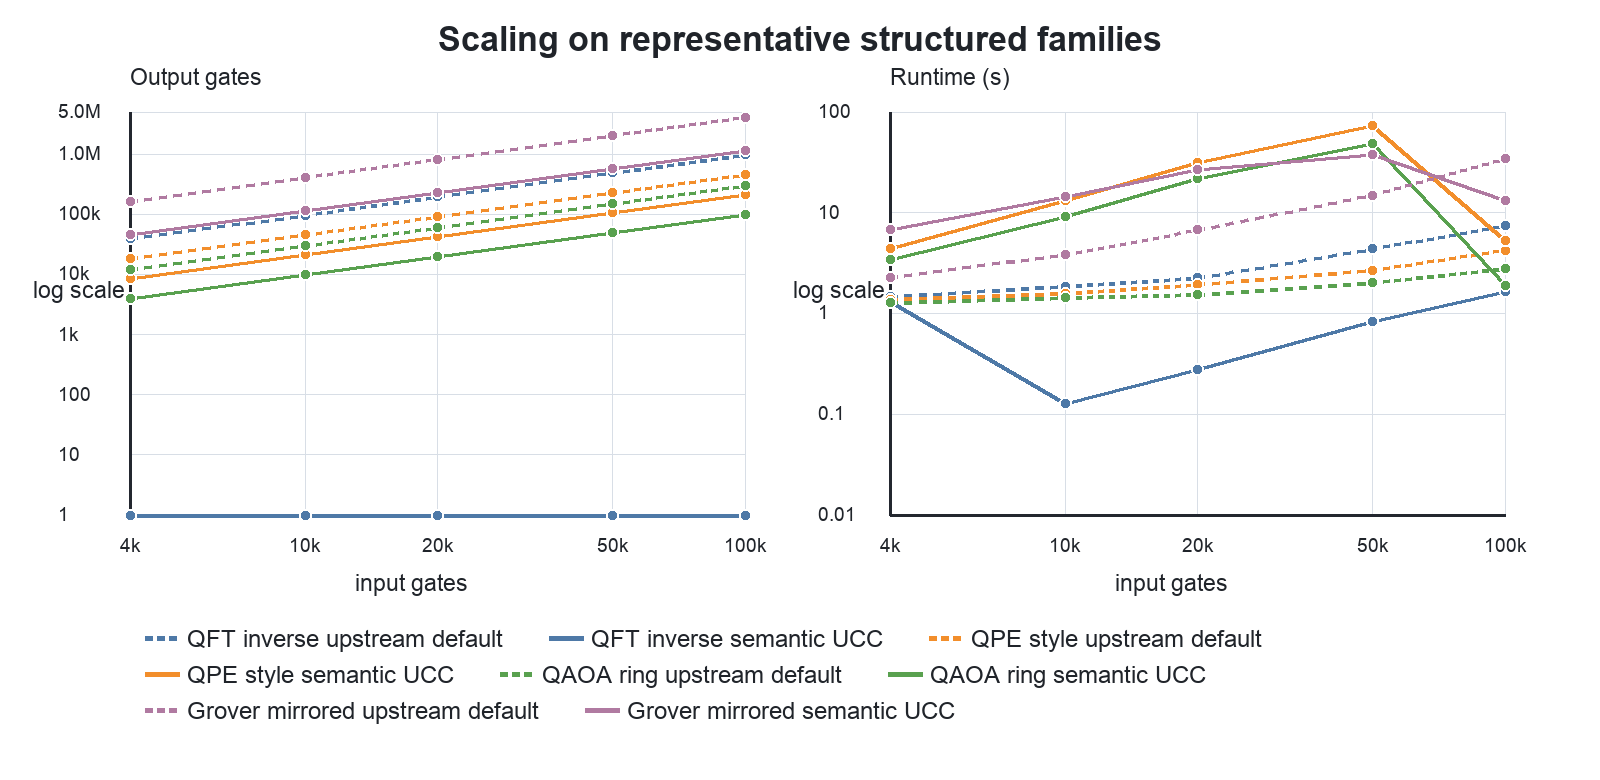
\includegraphics[width=\textwidth]{figures/scaling_plot.png}}{\fbox{\parbox{0.9\textwidth}{\centering\vspace{2em}Missing file: \texttt{figures/scaling\_plot.png}.\vspace{2em}}}}
\caption{Scaling behavior on representative structured families. Left: output gate count versus input gate count for upstream default (baseline UCC) and the semantic UCC artifact. Right: runtime versus input gate count. The semantic path preserves clear quality advantages across scale, while runtime behavior remains family-dependent.}
\label{fig:scaling}
\end{figure*}

\subsection{Scaling and Ablation}

The main scaling trends are summarized in \cref{fig:scaling}. The size sweep
covers $4$k, $10$k, $20$k, $50$k, and $100$k inputs for QFT-inverse,
QPE-style, QAOA-ring, and mirrored-Grover families; the QAOA-ring block uses
20 qubits. The most important
observations are stable quality behavior across scale and improving
repeated-family runtime once the semantic representation and dispatch controller are
enabled. The method is most effective on exact or highly repeated structure:
\texttt{qft\_inverse} remains maximally strong across all tested sizes,
\texttt{qpe\_style} remains a strong positive fixed-basis case,
\texttt{qaoa\_ring} consistently avoids UCC inflation, and the mirrored-Grover
family continues to match Qiskit quality at $100$k while remaining
more expensive. Direct spot checks on the semantic artifact give
\texttt{qpe\_style} $=82{,}200$ gates at $50$k in $2.504$ s and $164{,}400$
gates at $100$k in $4.636$ s, reflecting the phase-ladder plus
repeated-run controller improvements.

The non-monotonic semantic runtime between the $20$k and $50$k points is a
dispatch effect visible in the implementation, not an inferred hardware
effect. The 20,000-gate full-preset limit
\path{_MAX_FULL_PRESET_REFERENCE_SIZE} allows the 19,998-gate input to enter
the full preset-reference comparison,
whereas the 49,998-gate input exceeds that threshold and uses the cheaper
repeated-prefix/hierarchical route. The corresponding canonical witness
runtimes are 28.314~s and 20.934~s. This threshold explains the local drop;
it is not evidence of asymptotically decreasing compilation time.

The ablation picture is narrow. The dominant practical component is
conservative candidate control on recoverability-sensitive families, most
clearly on the 10,000-input-gate \texttt{qaoa\_ring} row, where the full configuration returns
$10{,}000$ gates while the no-candidate-selection variant returns $30{,}055$.
By contrast, \texttt{qft\_inverse}, \texttt{qft\_control},
\texttt{qpe\_style}, and \texttt{grover\_mirrored} are less sensitive to the
removal of individual structural rules. This reinforces the paper's current
framing: the main contribution is a bounded semantic representation and
dispatch controller that preserve recoverability before flat materialization,
rather than a single local identity.
